\documentclass[tikz]{standalone}
\usepackage{bm}
\newcommand{\vect}{\bm}
\newcommand{\del}{\boldsymbol{\nabla}}

\newcommand{\trans}[1]{{#1^\star}}
\newcommand{\surface}{h}
\newcommand{\shellcmd}[1]{\texttt{#1}}
\newcommand{\diffusioncoeff}{\mathcal{D}}
\newcommand{\exner}{\Pi}

\begin{document}
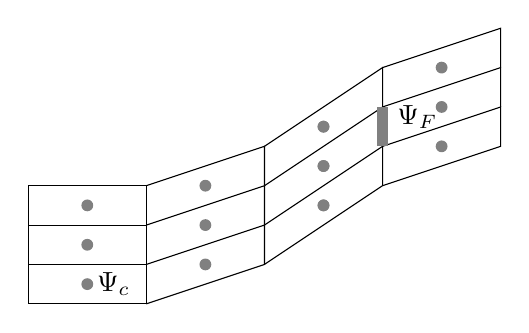
\begin{tikzpicture}[
  scale=0.5,
  cpnt/.style={fill=gray},
]
\draw (0,0) -- (3,0) -- (3,1) -- (0,1) -- (0,0);
\draw (0,1) -- (3,1) -- (3,2) -- (0,2) -- (0,1);
\draw (0,2) -- (3,2) -- (3,3) -- (0,3) -- (0,2);

\draw (3,0) -- (6,1) -- (6,2) -- (3,1);
\draw (6,2) -- (6,3) -- (3,2);
\draw (6,3) -- (6,4) -- (3,3);

\draw (6,1) -- (9,3) -- (9,4) -- (6,2);
\draw (9,4) -- (9,5) -- (6,3);
\draw (9,5) -- (9,6) -- (6,4);

\draw (9,3) -- (12,4) -- (12,5) -- (9,4);
\draw (12,5) -- (12,6) -- (9,5);
\draw (12,6) -- (12,7) -- (9,6);

\draw[line width=4, gray] (9,4) -- (9,5) node [pos=0.75,right,black] {$\Psi_F$};

\path [cpnt] (1.5,0.5) circle [radius=0.15] node [right] {$\Psi_c$};
\path [cpnt] (1.5,1.5) circle [radius=0.15];
\path [cpnt] (1.5,2.5) circle [radius=0.15];

\path [cpnt] (4.5,1) circle [radius=0.15];
\path [cpnt] (4.5,2) circle [radius=0.15];
\path [cpnt] (4.5,3) circle [radius=0.15];

\path [cpnt] (7.5,2.5) circle [radius=0.15];
\path [cpnt] (7.5,3.5) circle [radius=0.15];
\path [cpnt] (7.5,4.5) circle [radius=0.15];

\path [cpnt] (7.5,2.5) circle [radius=0.15];
\path [cpnt] (7.5,3.5) circle [radius=0.15];
\path [cpnt] (7.5,4.5) circle [radius=0.15];

\path [cpnt] (10.5,4) circle [radius=0.15];
\path [cpnt] (10.5,5) circle [radius=0.15];
\path [cpnt] (10.5,6) circle [radius=0.15];

\end{tikzpicture}
\end{document}
